\section{Opgave 1}
\subsection{Beskrivelse og Design}

\subsection{Programtest}
	For at teste at dette program virker som forventet er det nødvendigt at teste følgene:
 	\begin{enumerate}
 		\item Programmet håndterer hver dekade korrekt og lægger dekader korrekt sammen
 		\item Programmet håndterer fejl-input uden at bryde sammen og at det genkender exit kommandoen
 	\end{enumerate}
 	For at teste at programmet håndterer hver dekade op til 100.000.000 som er den højeste dekade programmet har et romersk numeral for, er der inkluderet en metode kaldet $testDecades$ i klassen $RomanNumerals$ som tilgås ved at indtaste den skjulte kommando "test" i konsollen. Resultatet af dette ses nedenfor som et screenshot da listings pakken til latex ikke kan håndtere unicode karakteren for et overstreget bogstav.
 	\begin{figure}[h]
 	
 	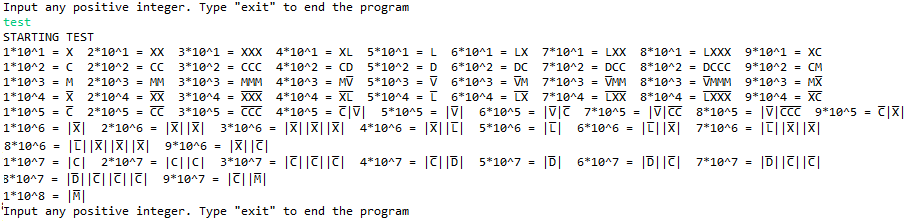
\includegraphics[scale=0.8]{test_opgave_1.png}
 	\caption{Output fra testDecade metoden}
	
	\end{figure}
	\begin{lstlisting}
Input any positive integer. Type "exit" to end the program
test
STARTING TEST
1*10^1 = X  2*10^1 = XX  3*10^1 = XXX  4*10^1 = XL  5*10^1 = L  6*10^1 = LX  7*10^1 = LXX  8*10^1 = LXXX  9*10^1 = XC  
1*10^2 = C  2*10^2 = CC  3*10^2 = CCC  4*10^2 = CD  5*10^2 = D  6*10^2 = DC  7*10^2 = DCC  8*10^2 = DCCC  9*10^2 = CM  
1*10^3 = M  2*10^3 = MM  3*10^3 = MMM  4*10^3 = MV̅  5*10^3 = V̅  6*10^3 = V̅M  7*10^3 = V̅MM  8*10^3 = V̅MMM  9*10^3 = MX̅  
1*10^4 = X̅  2*10^4 = X̅X̅  3*10^4 = X̅X̅X̅  4*10^4 = X̅L̅  5*10^4 = L̅  6*10^4 = L̅X̅  7*10^4 = L̅X̅X̅  8*10^4 = L̅X̅X̅X̅  9*10^4 = X̅C̅  
1*10^5 = C̅  2*10^5 = C̅C̅  3*10^5 = C̅C̅C̅  4*10^5 = C̅|V̅|  5*10^5 = |V̅|  6*10^5 = |V̅|C̅  7*10^5 = |V̅|C̅C̅  8*10^5 = |V̅|C̅C̅C̅  9*10^5 = C̅|X̅|  
1*10^6 = |X̅|  2*10^6 = |X̅||X̅|  3*10^6 = |X̅||X̅||X̅|  4*10^6 = |X̅||L̅|  5*10^6 = |L̅|  6*10^6 = |L̅||X̅|  7*10^6 = |L̅||X̅||X̅|  8*10^6 = |L̅||X̅||X̅||X̅|  9*10^6 = |X̅||C̅|  
1*10^7 = |C̅|  2*10^7 = |C̅||C̅|  3*10^7 = |C̅||C̅||C̅|  4*10^7 = |C̅||D̅|  5*10^7 = |D̅|  6*10^7 = |D̅||C̅|  7*10^7 = |D̅||C̅||C̅|  8*10^7 = |D̅||C̅||C̅||C̅|  9*10^7 = |C̅||M̅|  
1*10^8 = |M̅|  
	\end{lstlisting}
	Herefter testes om programmet kan kombinere tal i flere dekader. Resultatet af testen ses nedenfor.
	\begin{lstlisting}[caption=Test af dekadekombination]
Input any positive integer. Type "exit" to end the program
1337
MCCCXXXVII
	\end{lstlisting}
	Hvilket er korrekt. \\
	\\
	Til sidst testes punkt nr. 2, at programmet afbrydes når brugeren indtaster "exit" kommandoen.
	\begin{lstlisting}[caption=Test af exit kommando]
Input any positive integer. Type "exit" to end the program
exit
Done!
	\end{lstlisting}
	Og at det kan håndtere input af negative tal samt ikke-tal.
	\begin{lstlisting}[caption=Test af dårligt input]
Input any positive integer. Type "exit" to end the program
-42
Please enter a positive integer, that's a number without a decimal point,larger than zero
Input any positive integer. Type "exit" to end the program
NaN
Please enter a positive integer, that's a number without a decimal point,larger than zero
Input any positive integer. Type "exit" to end the program
	\end{lstlisting}
	
	Disse tests opnår 100\% kode dækning. Selvom dette selvfølgelig ikke er en garanti for at programmet altid vil virke vil vi ikke gå videre med tests da det ville kræve at teste alle tænkelige input, hvilket er umuligt med den tid vi har til rådighed. Yderligere er programmet ikke begrænset af integer overflow, så dette er ikke testet.